%%%%%%%%%%%%%%%%%%%%%%%%%%%%%%%%%%%%%%%%%%%%%%%%%%
\section{Asymptotic analysis of PDE system}
%%%%%%%%%%%%%%%%%%%%%%%%%%%%%%%%%%%%%%%%%%%%%%%%%%

%%%%%%%%%%%%%%%%%%%%%%%%%%%%%%%%%%%%%%%%%%%%%%%%%%
\subsection{Numerical observation of traveling waves}
%%%%%%%%%%%%%%%%%%%%%%%%%%%%%%%%%%%%%%%%%%%%%%%%%%

%%%%%%%%%%%%%%%%%%%%%%%%%%%%%%%%
\begin{figure}[htbp]
  \centering
  \label{fig:numericalTWave}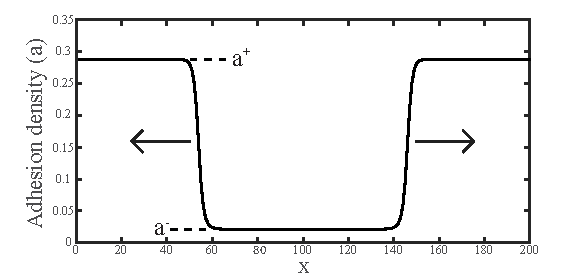
\includegraphics[width=13cm]{figs/figawave.pdf}
  \caption{Numerical observation of traveling wave.}
\end{figure}
%%%%%%%%%%%%%%%%%%%%%%%%%%%%%%%%
Figure~\ref{fig:numericalTWave}


%%%%%%%%%%%%%%%%%%%%%%%%%%%%%%%%%%%%%%%%%%%%%%%%%%
\subsection{Transformation into traveling coordinate $z$ and matched asymptotic analysis}
%%%%%%%%%%%%%%%%%%%%%%%%%%%%%%%%%%%%%%%%%%%%%%%%%%


\begin{align}
\dfrac{\partial a}{ \partial t}  & =  f(a,y)\\
0 & =g \left(a,y,\dfrac{\partial^2 y}{\partial x^2}\right).
\end{align}

 \text{A narrow version of the system is obtained if we assume the force balance equations are linear in $a$}
\begin{align}
\dfrac{da}{ dt}  & = f_1(y) - a f_2(y)\label{eq::gen_a}\\
0 & = g_1(y) - ag_2(y) +  \dfrac{\partial^2 y}{\partial x^2}\label{eq::gen_ym}
\end{align}
\textbf{This can be obtained from our system given the following simplifying assumption.} Assume that the cortex does not move significantly during excitation, $y_C = y_C^{ss}$, leaving us with the new system of two equations:
\begin{align}
\dfrac{\partial a}{ \partial t}  & =  \dfrac{c^{ss}}{1+c^{ss}} \mbox{exp}\left(-\dfrac{y-y_C^{ss}}{D}\right) - a \mbox{exp} \left(\dfrac{y-y_C^{ss}}{F} \right)\label{eq::a_ODE}\\
0 & = -a(y - y_C^{ss}) + P (1-y) + \gamma_M \dfrac{\partial^2 y}{\partial x^2}\label{eq::yM_eq}
\end{align} 


Transform to wave coordinate $z = x-vt$ and~\ref{eq::gen_a} and~\ref{eq::gen_ym} become:
\begin{align}
-v \dfrac{da}{ dz}  & = f_1(y) - a f_2(y)\label{eq::gen_a_z}\\
0 & = g_1(y) - ag_2(y) +  \dfrac{\partial^2 y}{\partial z^2}\label{eq::gen_ym_z}
\end{align}
We can use Eq.~\ref{eq::gen_ym_z} to solve for $a$:
\begin{flalign}
 a = \dfrac{1}{g_2(y)} \left( g_1(y) + \dfrac{\partial^2 y}{\partial z^2} \right)
\end{flalign}
Then it follows that:
\begin{equation}\Rightarrow  -v \dfrac{\partial a}{ \partial z}   =  f_1(y)  -  \dfrac{g_1(y)}{g_2(y)}f_2(y) - \dfrac{f_2(y)}{g_2(y)} \dfrac{\partial^2 y}{\partial z^2}\label{eq::ODE_z}
\end{equation}

%%%%%%%%%%%%%%%%%%%%%%%%%%%%%%%%
\begin{figure}[htbp]
  \centering
  \label{fig:multiscaleRegimes}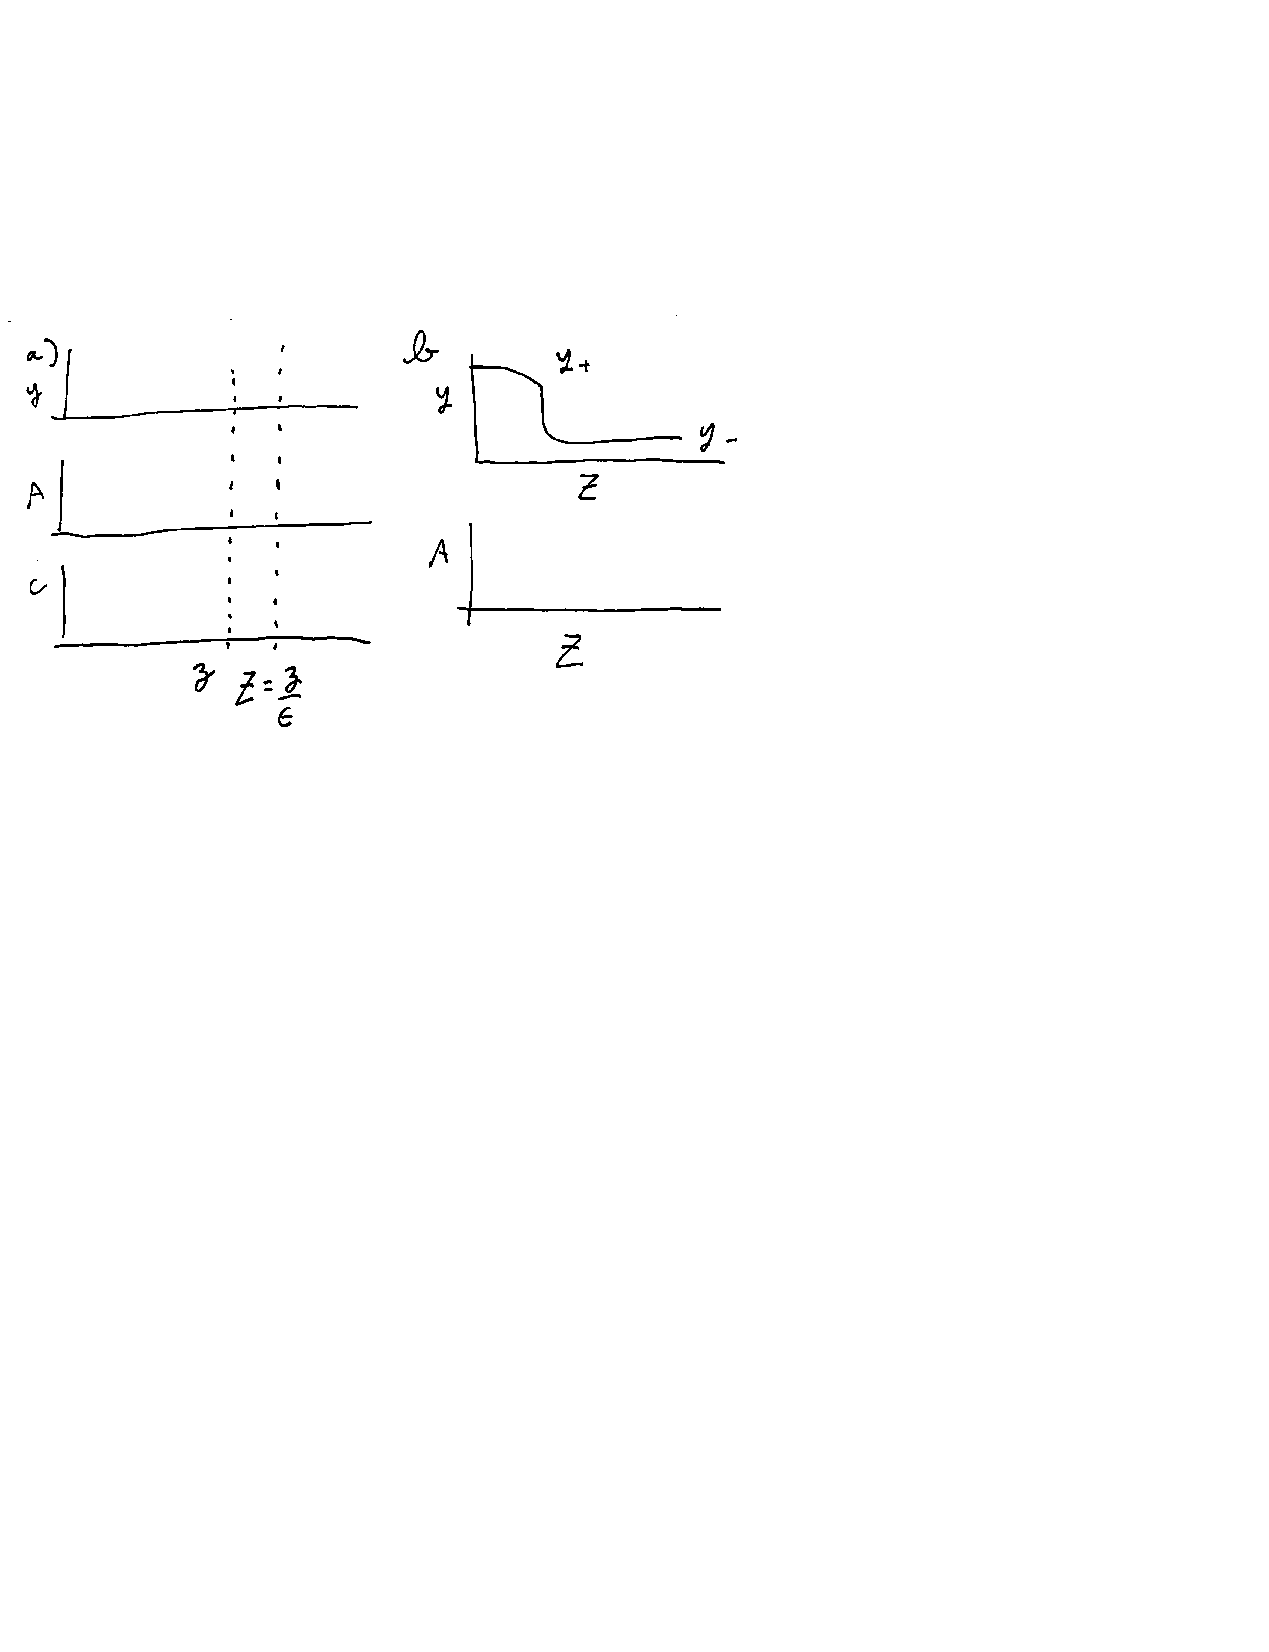
\includegraphics[width=13cm]{figs/figMultiscaleRegimes.pdf}
  \caption{Decomposition of PDE solution into a traveling wave with regimes in different scales.}
\end{figure}
%%%%%%%%%%%%%%%%%%%%%%%%%%%%%%%%
Figure~\ref{fig:multiscaleRegimes}


%%%%%%%%%%%%%%%%%%%%%%%%%%%%%%%%%%%%%%%%%%%%%%%%%%
\subsection{Non-local Maxwell Condition for traveling waves}
%%%%%%%%%%%%%%%%%%%%%%%%%%%%%%%%%%%%%%%%%%%%%%%%%%

%%%%%%%%%%%%%%%%%%%%%%%%%%%%%%%%
\begin{figure}[htbp]
  \centering
  \label{fig:NLMC}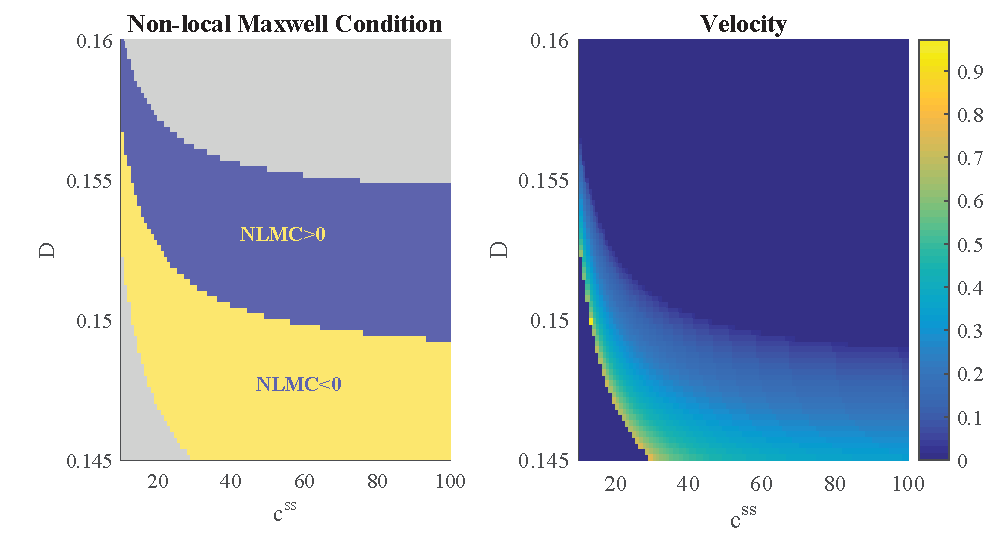
\includegraphics[width=13cm]{figs/NLMC1.pdf}
  \caption{Nonlocal Maxwell condition demonstrating emergence of traveling waves.}
\end{figure}
%%%%%%%%%%%%%%%%%%%%%%%%%%%%%%%%
\ref{fig:NLMC}
